\section{Literature review}\label{sec:review}
In this chapter, previous work on the optimization of network tied-arch bridges is summarized. In Section \ref{sec:rev_arr} it is shown how the different hanger arrangements evolved and which objectives are considered aiming to determine an optimal arrangement. Fundamentally, two approaches are taken for this investigation. On the one hand, parametric studies allow determining the critical parameters. On the other hand, optimization methods have been used not just to identify the tendencies, but to optimize the choice of parameters in the continuous domain. Few authors have taken a further step and introduced a design methodology allowing for a fast and approximately optimized design, which are presented in Section \ref{sec:rev_meth}. While it has received much attention for cable-stayed bridges, cable loss in network tied-arch bridges is only considered scarcely and isolated from the previously mentioned work.[As cen be deciding for design] The corresponding literature is summarized in Section \ref{sec:rev_cable}. Ultimately, the Master Thesis of Riccardo Cavegn, which builds the foundation of this Thesis, is summarized in Section \ref{sec:rev_prev} and a summary of this chapter is given in Section \ref{sec:rev_sum}.

\subsection{Hanger arrangements}\label{sec:rev_arr}
\paragraph*{Hanger unloading}
Per Tveit, described the concept of network tied-arch bridges in his dissertation in 1959. He designed two of the first bridges of this type in 1963 in Norway. In these early stages, only the parallel hanger net and the constant change of inclination pattern are used. Since then, he has been giving lectures around the world to contribute to the broader use of network tied-arch bridges. He points out the various advantages over vertical hangers in terms of lower steel weights, simple detailing and the good use of strong materials \citep{Tveit}. He recommends constant hanger spacing on the arch with one hanger per node to minimize the bending moments in the arch. In \cite{Tveit3} he also conducted investigations on the hanger arrangement, aiming to prevent hanger unloading which is a critical issue under asymmetric loading for short-span bridges. It is found that whereas flat inclinations are more suitable to prevent hanger unloading, they also result in higher hanger forces. To find a solution for these opposing objectives he developed a diagram, presented in Figure \ref{fig:Tveit2}, which predicts the maximum hanger inclination without hanger unloading depending on the ratio of life to dead loads and the loaded length. As a first optimization of the hanger arrangement, it is proposed to increase the inclinations of the hangers as much as possible before the first hanger unloading occurs.

\begin{figure}[H]
    \centering
    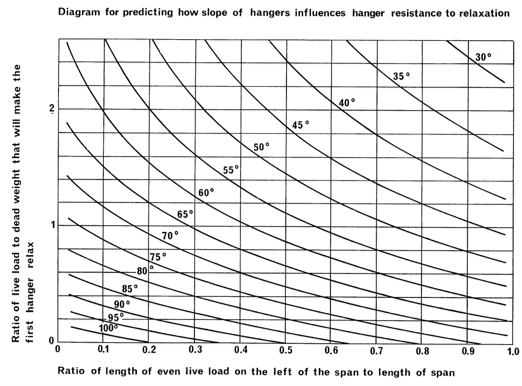
\includegraphics[width=0.6\textwidth]{Pictures/MaximumHangerInclination.png}
    \caption{Indication of the first hanger relaxation (adopted from \citep{Tveit3})}
    \label{fig:Tveit2}
\end{figure}

%Later, he proposed an arrangement with constant distances between the hanger connection points in the middle of the tie, as shown in \autoref{fig:Tveit}. While the nodes on the arch are spaced equidistantly, the connection points on the tie are constructed with the help of an inclined ellipse and an abscissa and an ordinate depending on the parameters $p_1$ and $p_2$. To determine the points on the tie, linearly spaced vertical lines are drawn to the ellipse. The locations of the nodes on the tie are then determined from the ordinate values of the intersection points.\\
%\begin{figure}[H]
%\centering
%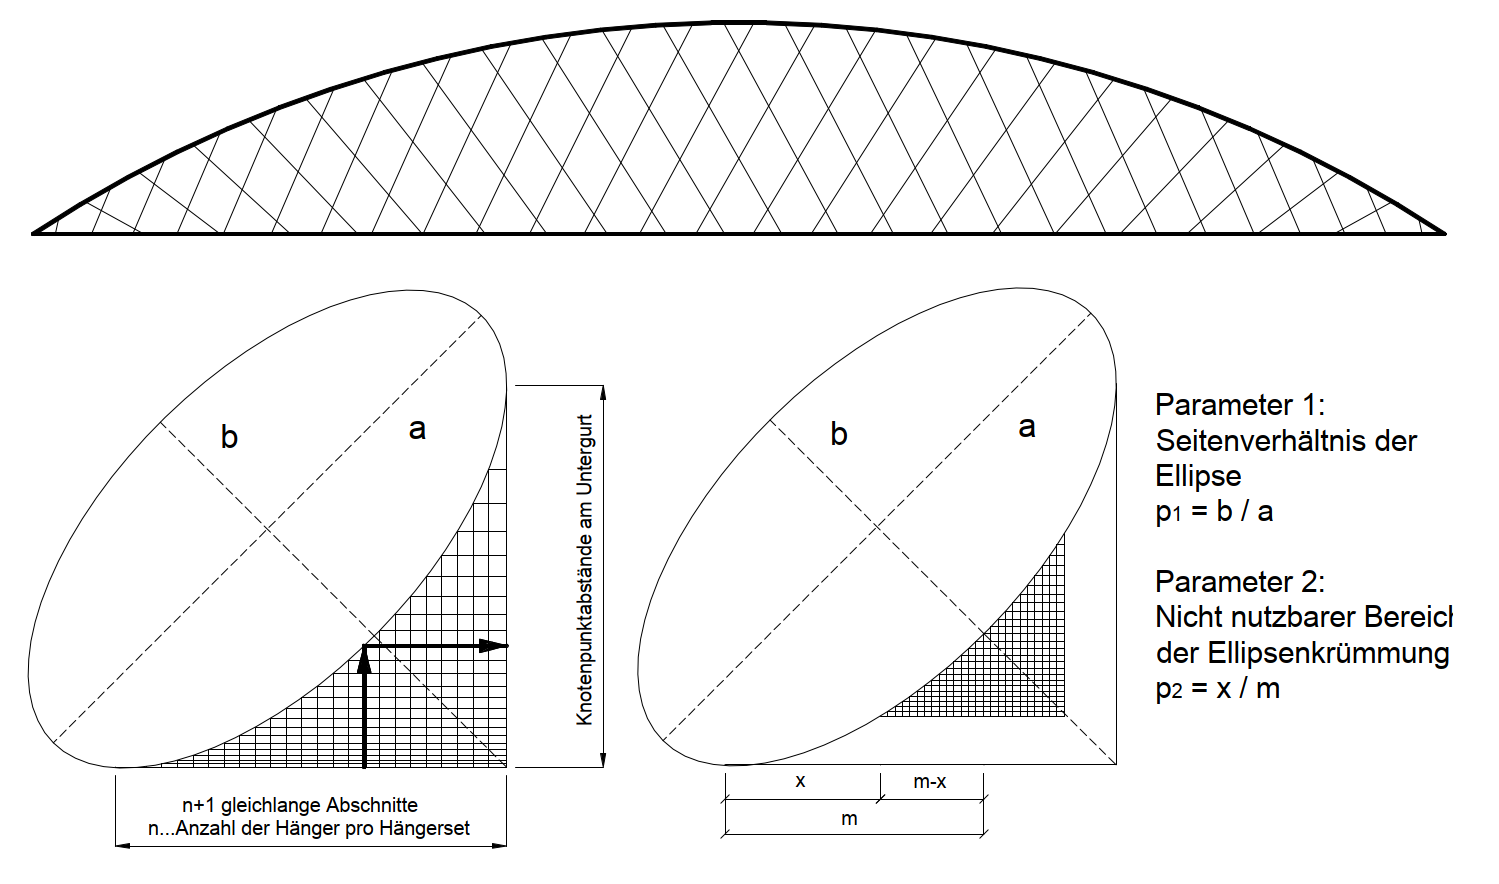
\includegraphics[width=0.7\textwidth]{Pictures/ArrangementTveit.PNG}
%\caption{Arrangement with constant distances in the middle of the tie (adopted from \cite{Teich}).}
%\label{fig:Tveit}
%\end{figure}

\paragraph*{I don't know}
In the new millennium, Tveit supervised multiple Master Theses aiming to optimize the design of network-tied arch bridges. In \citep{BrunnSchanack} [nochmals lesen was da genau gemacht wurde]. They developed the radial arrangement aiming to have a pattern which optimally complies with a circular arch. In the radial arrangement, the hangers are equally spaced on the arch and two following hangers cross each other symmetrically to the radius as shown in \autoref{fig:Brunn}. It was the intention, that if the hanger forces are uniform, the thrust line also approximately corresponds to a circle, resulting in an efficient use of the arch. In the literature, this arrangement is either described by the angle $\alpha$ between the arch and the hanger or by the angle $\beta$ between the hangers and the radius at the first intersection point.

\begin{figure}[H]
\centering
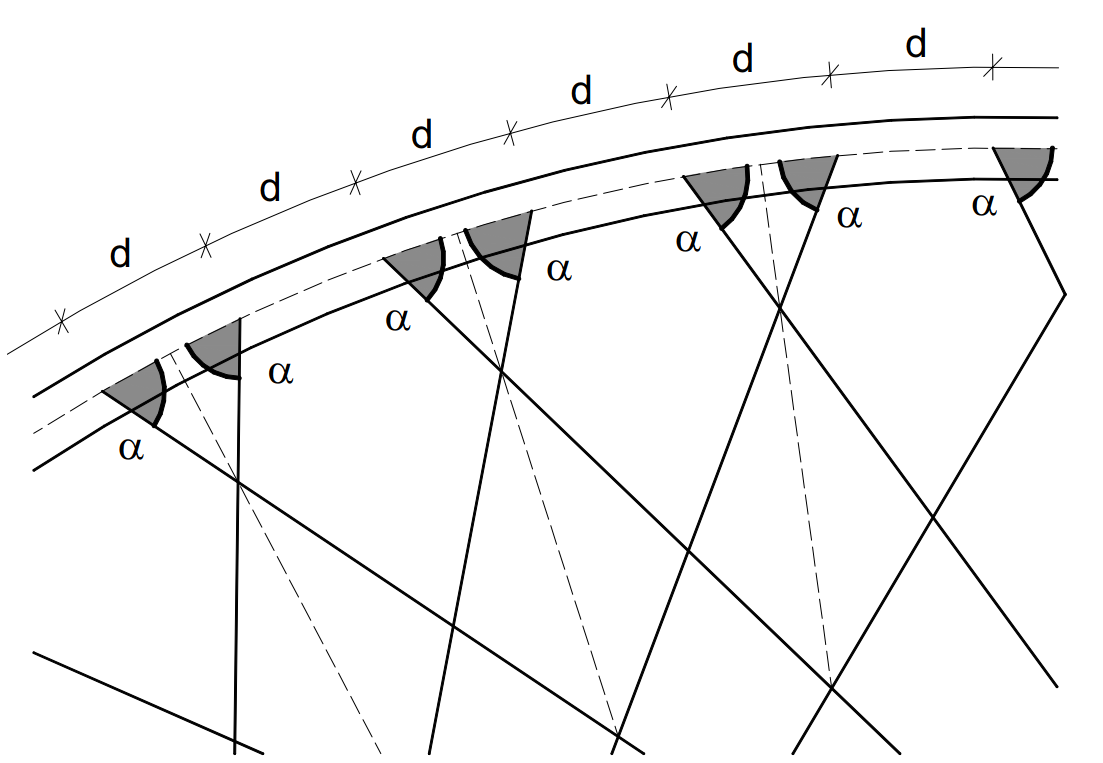
\includegraphics[width=0.4\textwidth]{Pictures/RadialArrangement.PNG}
\caption{Radial hanger arrangement (adopted from \citep{BrunnSchanack2}).}
\label{fig:Brunn}
\end{figure}

Both of the authors continued their work in the field of network tied-arch bridges and conclude their findings in \citep{BrunnSchanack2}. Besides the bending moments and the maximum hanger forces, also the variation of hanger forces, which are relevant for fatigue, and the elastic embedding of the arch is focused on. These objectives are evaluated manually/arbitrarily. In a comparison of the different hanger patterns, it is concluded that parallel hangers are disadvantageous concerning the bending moments in the arch as the hanger forces vary strongly. Angles of inclination between $55\degree$ and $60\degree$ give the best results. For the constant change of inclination arrangement the middle hanger was recommended to be inclined in the similar range from $56\degree$ to $60\degree$. Further, the change of inclination between two following hangers should lead to an inclination of up to $80\degree$ in the steepest hangers. The radial arrangement was considered optimal, especially for the small corresponding variation of maximum hanger forces and uniform embedding of the arch. The angle between the hangers and the arch are recommended to be between $55\degree$ and $60\degree$. Interestingly, the optimal solutions for each hanger arrangement feature a middle hanger with an inclination of $55\degree$ to $60\degree$. Further, it is recommended that the hanger spacing on the arch lies between \SI{2.5}{m} and \SI{4}{m}.

\paragraph*{Hanger forces}
To judge the objectives mathematically \citep{Teich} conducted a vast parameter study varying the key in-plane parameters. Its focus lies on the objectives related to the hangers which are combined into a scaled dimensionless score. Namely, these objectives are the maximum force and its variation, the cyclic stresses and the amount of unloaded cables. In the evaluation of these objectives the three hangers closest to the arch were disregarded for and it is proposed to design them detached from the general hanger pattern. The parameters such as the span, the rise, the amount of hangers and their arrangement are varied in the study, leading to a total of approximately 90000 variants. The only in-plane parameter that is left constant is the arch shape which is always modelled circular. Based on the normalized and combined results, a design methodology was developed which is explained in Section \ref{sec:rev_meth}. For the parallel hanger pattern smaller angles of inclination between $50\degree$ and $55\degree$ are recommended. However, hanger unloading poses a serious issue for this arrangement. The constant change of inclination arrangement generally relies on large changes of the inclination and yields the best results with respect to the cyclic stresses and hanger unloading. The radial arrangement performed well in all objectives, especially if the amount of hangers is rather low. It gave the best results overall and Teich recommends intersection angles around $36\degree$. For some cases also the arrangement with equidistant spacing on the tie proofed efficient. In this pattern, optimal results were obtained by a variety of values for the two parameters.
%results normalized and mixed multiple times.
%no prestressing
\paragraph*{Fatigue}
The assumption that the hangers close to the knuckles should be designed independently from the overall pattern agrees with \citep{Pellegrino}. In this study various hanger patterns are evaluated with respect to fatigue. The considered hanger patterns are the constant change of slope and the radial arrangement which are also compared to an arrangement with vertical hangers. It is found that with respect to the cyclic stresses, vertical hangers are superior over network arrangements. By inclining the vertical hangers the behaviour deteriorates strongly and improves again for flat inclinations. Especially the flat hangers near the knuckle undergo very high cyclic stresses and various arrangements to improve this issue are studied. However, none of the adapted arrangements provided better results independent of the intersecting angle. Steeper hangers near the knuckles are generally a good advice to start with. For a radial hanger arrangement with an intersecting angle of $35\degree$, it is recommended to arrange the last five hangers of each set parallel to the previous one, as shown in \autoref{fig:Pellegrino}. This advice has to be judged considering that a high amount of 22 hangers per set without prestressing were used in the study.

\begin{figure}[H]
    \centering
    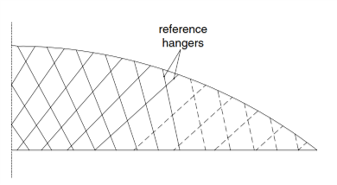
\includegraphics[width=0.5\textwidth]{Pictures/PellegrinoArrangement.png}
    \caption{Modified radial arrangement (adapted from \citep{Pellegrino})}
    \label{fig:Pellegrino}
\end{figure}

\paragraph*{Numerical optimization}
Recently, many researchers have focused on numerical optimization methods over parametric studies. Technically, all parameters describing the scheme of a network tied arch bridge can be considered. However, as it is usually not the aim to optimize the entire design process, researchers prefer to limit the process to a few key variables. As some of the parameters are of discrete form, the problem is mathematically described as a constrained mixed-integer problem. Genetic algorithms with penalization provide an efficient and often used tool for these problems. In \citep{Belevicius}, an optimal pedestrian bridge scheme with respect to weight minimization is obtained for different spans. Even with the rather limited amount of nine parameters, the optimized sets are well dispersed over the feasible domain, illustrating the multi-modality of the underlying problem.
It also demonstrates well the difficulties associated with numerical optimization for design purposes. Even after reducing the amount of parameters, the results do not resemble typical tied-arch bridges, be it for the high amount of hangers or the large rise-to-span ratio. The aim of finding a simple and fast method for obtaining the full initial design is therefore reached only in an unsatisfactory manner. Ultimately, It a strongly varying hanger pattern is recommended as well as a rise-to-span ratio of 0.2 to 0.23. The hanger spacing on the tie should be shorter for the steep hangers and increase towards the other side.\\

In \citep{Tan} a pedestrian bridge with a sparse hanger arrangement was investigated using an evolutionary optimization procedure. Each hanger is arranged independently of an overall arrangement. It was found that an arrangement approximately consisting of two separate patterns reduced the internal forces in the arch and the tie the most. Near the knuckles vertical hangers and in the span approximately parallel hangers resulted as shown in \autoref{fig:Tan}.

\begin{figure}[H]
\centering
\begin{subfigure}{0.5\textwidth}
    \centering
    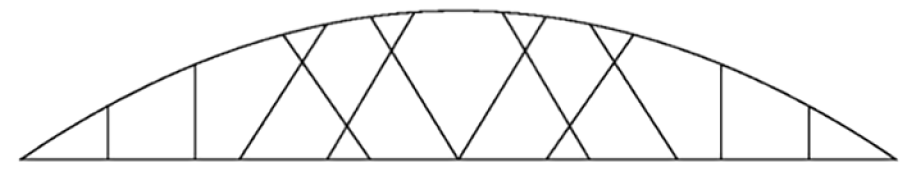
\includegraphics[width=0.9\textwidth]{Pictures/Tan 1.PNG}
\end{subfigure}%
\begin{subfigure}{.5\textwidth}
    \centering
    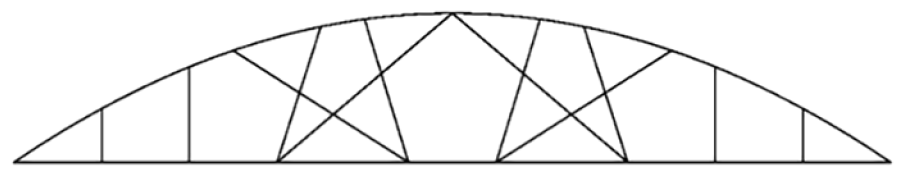
\includegraphics[width=0.9\textwidth]{Pictures/Tan 2.PNG}
\end{subfigure}
\caption{Optimal sparse hanger arrangements (adopted from \cite{Tan}).}
\label{fig:Tan}
\end{figure}

%[Ostrycharczyk] %Adapted radial pattern for equidistant hanger spacing on tie. Highly important that hangers don't lie to close to each other on the arch.


\subsection{Design methodology} \label{sec:rev_meth}

In a first step the number of hangers is chosen according to the recommended values shown in [Figure]. Using the amount of hangers and the span the optimal hanger arrangement pattern is chosen using a different table. For all cases either the constant change of inclination or the radial arrangement are the preferred choice. In Tables corresponding to the hanger arrangement pattern the best set of parameters can be chosen depending on the amount of hangers. An example for the radial arrangement is shown in [Figure]. The three hangers closest to the knuckle should ultimately be designed manually. They were also excluded in the evaluation of the objectives.
%[Bruno]
%[Teich]

\subsection{Cable loss} \label{sec:rev_cable}
Most of the work dedicated on cable loss focuses on cable-stayed bridges. There, it is not unusual for this accidental limit state to govern the design of the superstructure. In \citep{Wolff} is found that the loss of two or more cables can impair the global stability of a cable-stayed bridge.
[give guidelines for cable-stayed bridges?]
In \citep{Zoli} a parametric sensitivity study on cable loss for the Blennerhassett Island Bridge is conducted. [Kann man diese Publikation irgendwo finden?]
It is concluded that cable loss should be a key consideration for the design process for all major bridges.\\

In \citep{Bruno}, a study on the behaviour of network tied-arch bridges is conducted to identify the key factors on the impacts. The behaviour is studied using the simplified approaches of the PTI and the Eurocode and compared to a dynamic non-linear FE-analysis. As a base case, a bridge with a span of \SI{180}{m} and a rise of \SI{30}{m} is studied featuring a parallel hanger arrangement with 17 hangers per set and an inclination of $65 \degree$. Whereas the prestressing is taken into account using the "zero-displacement method"/the methodology by Bruno.

It was found that the most dangerous cables to lose are the ones located near the quarter points of the tie and inclined towards the middle of the arch. The corresponding vertical displacements are maximal for this hanger with a value of $l/4000$. The stresses in the neighbouring hangers of the same set increase by 60\% if the cable at the quarter point is lost. The hangers of the other set are less affected increasing by a maximum of less than 25\% as shown in Fig. \ref{fig:Bruno}. Further, he found that parallel arrangements with flatter inclinations cause the displacements and the internal forces to increase. Restricted to the plausible range of $50\degree$ to $70\degree$ differences amounting up to 20\% can be expected. In Figure [] the respective displacements are also compared to the arrangement with vertical hangers, where also the resulting total volumes of the hangers are given. It is seen that the vertical arrangement performs much butter despite using a smaller amount quantity of cable material. Overall it is concluded that also the simplified methods provide an adequate degree of accuracy.

\begin{figure}[H]
    \centering
    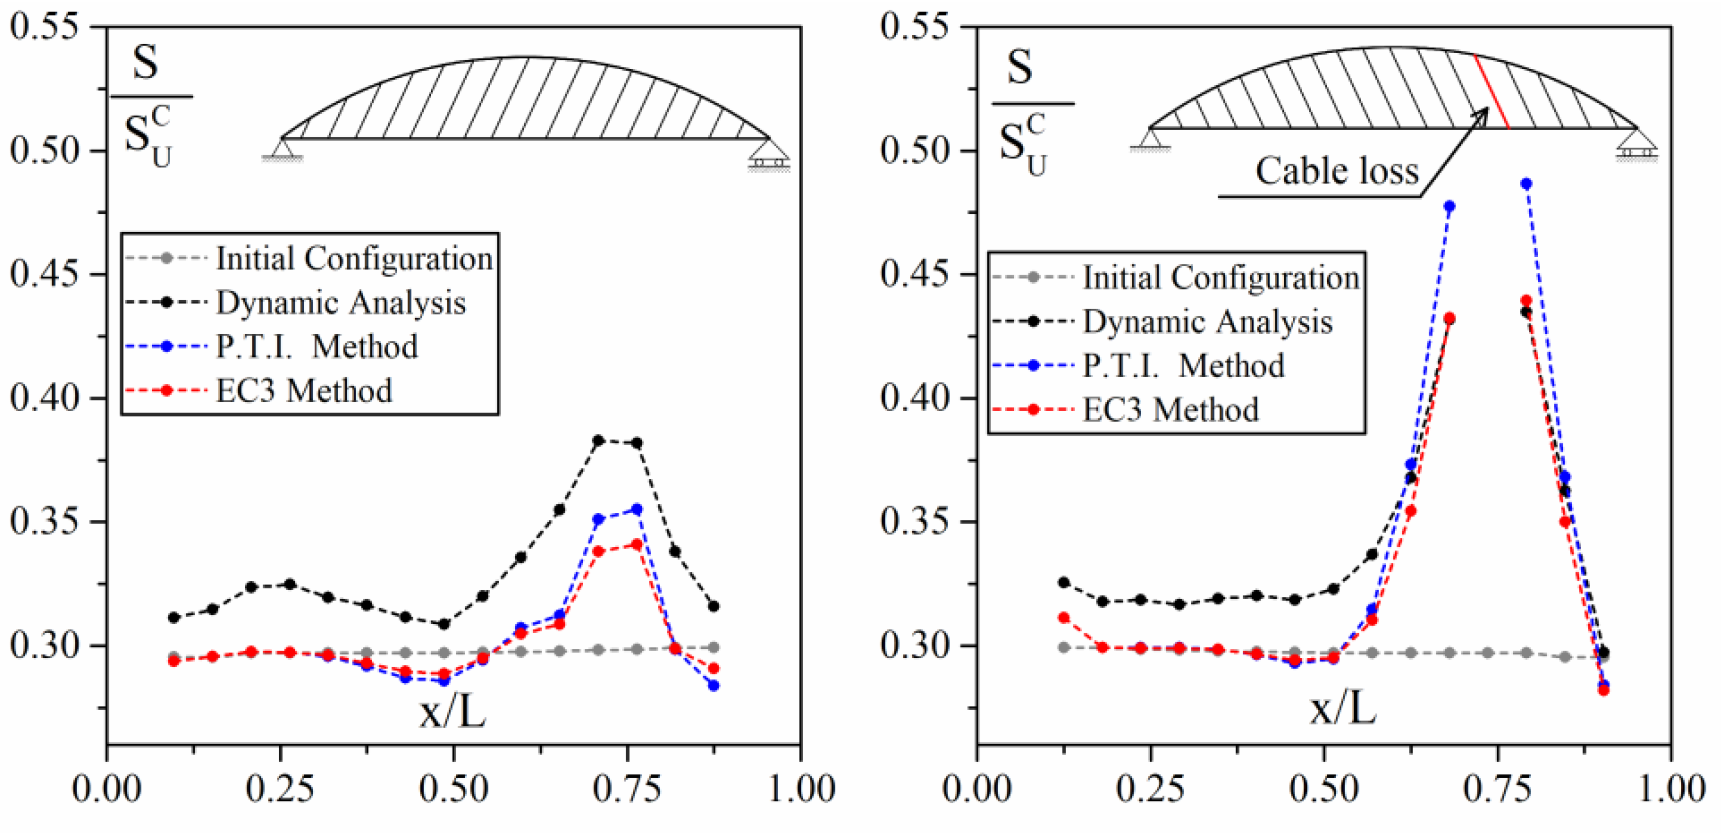
\includegraphics[width=0.75\textwidth]{Pictures/BrunoCableLoss.PNG}
    \caption{Stress distribution in the hanger sets (adopted from \citep{Bruno})}
    \label{fig:Bruno}
\end{figure}

\begin{figure}[H]
    \centering
    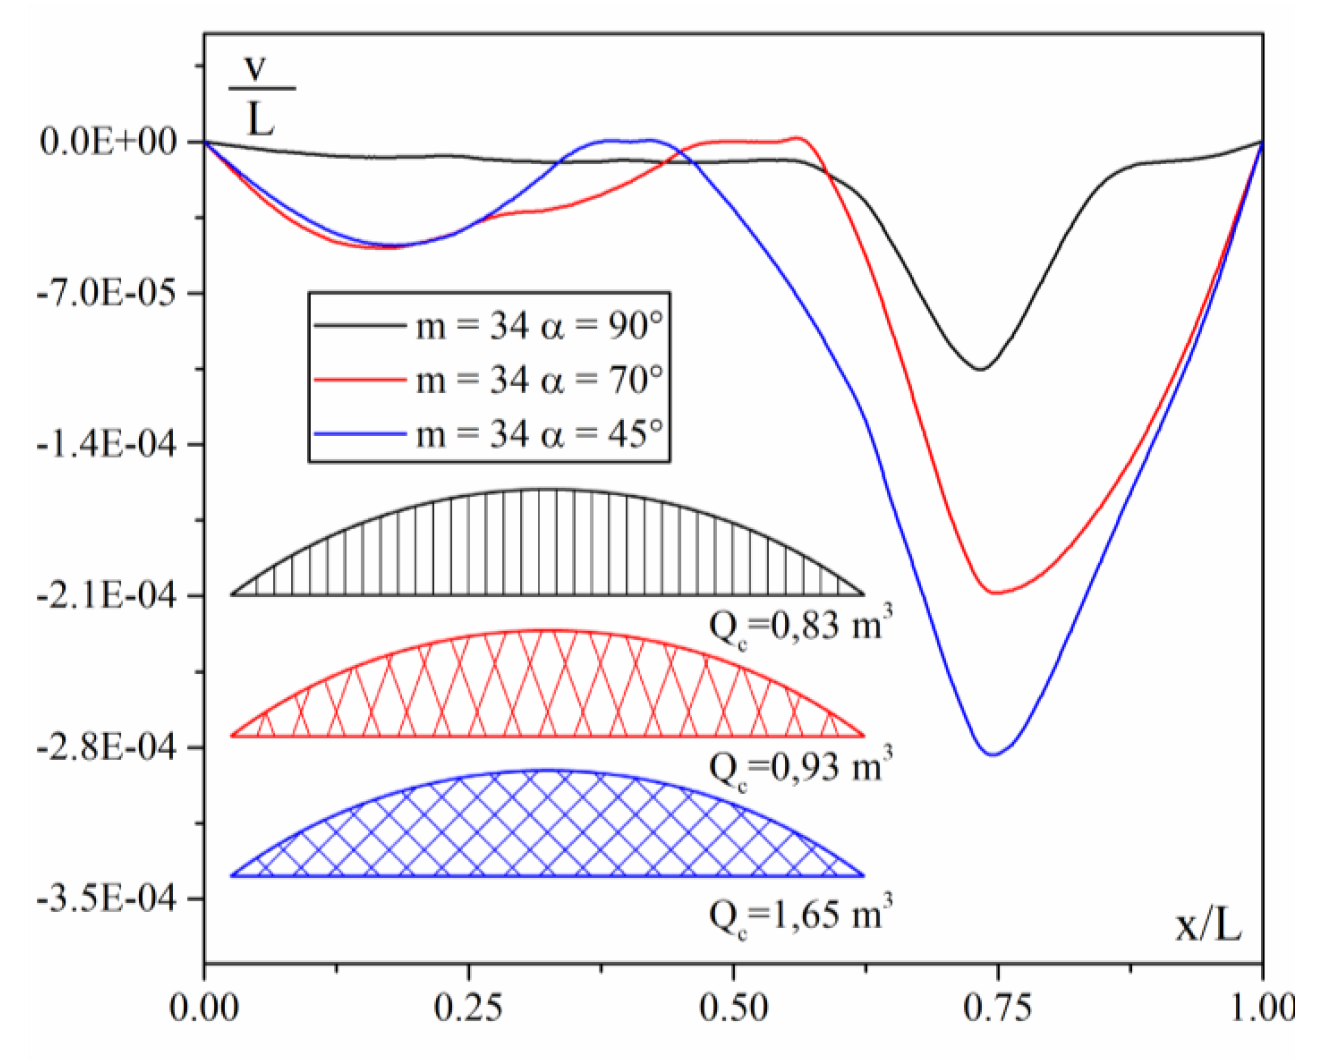
\includegraphics[width=0.6\textwidth]{Pictures/BrunoArrangements.PNG}
    \caption{Comparison between vertical and network cable systems (adopted from \citep{Bruno})}
    \label{fig:Bruno2}
\end{figure}

%[Islam] Considers material costs agrees with optimal inclination

\newpage
\subsection{Previous work in this series}\label{sec:rev_prev}
In a previous Master's Thesis at the Chair of Structural Engineering for Concrete Structures and Bridge Design, Riccardo Cavegn investigated the optimal arch geometry \citep{Cavegn}. Its dependency on the hanger arrangement was studied in particular with the Blennerhassett Island Bridge as a reference bridge. As a hanger pattern, the constant change of inclination arrangement was investigated in a parameter study. Two examples are shown in Fig. \ref{fig:Cavegn1} and Fig. \ref{fig:Cavegn2}, the latter corresponds to the special case of a parallel hanger pattern with parallel hangers.

\begin{figure}[H]
\centering
\begin{subfigure}{0.5\textwidth}
    \centering
    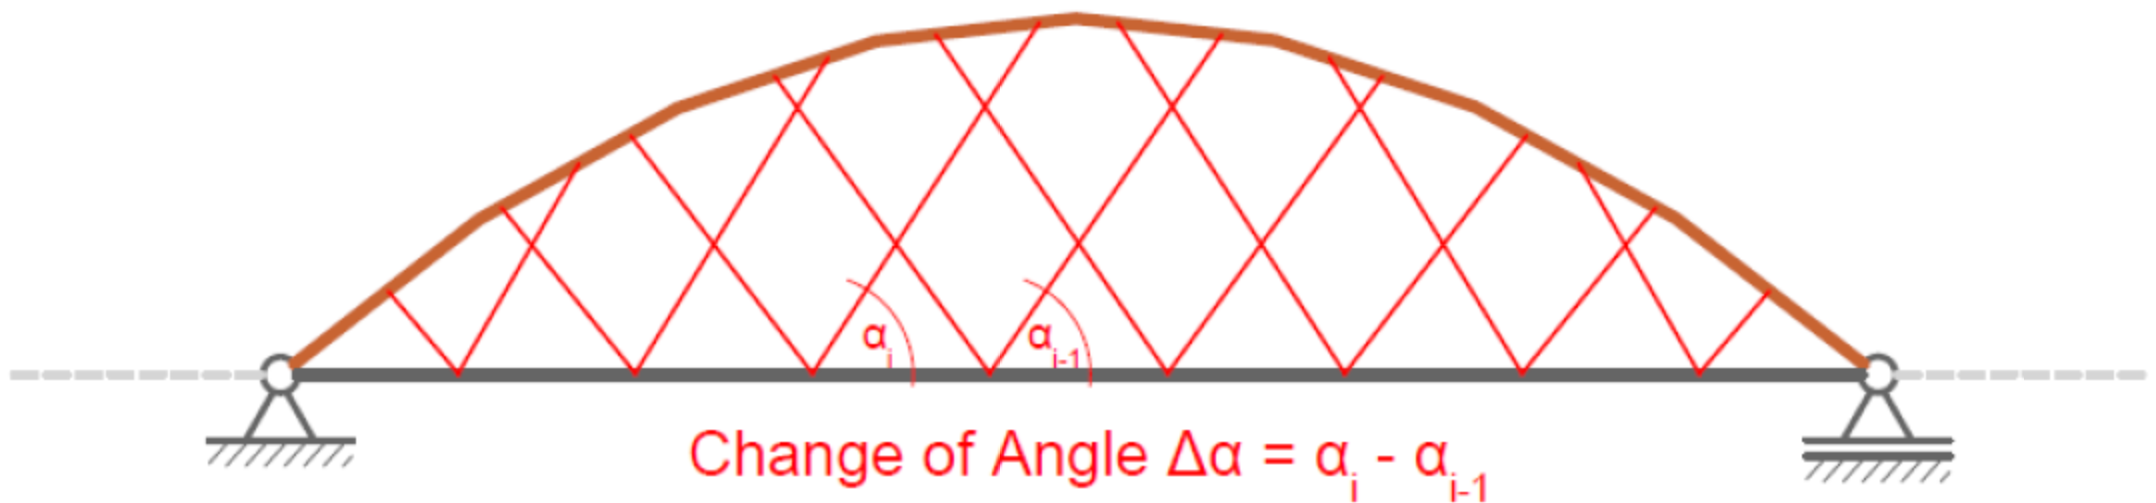
\includegraphics[width=0.9\textwidth]{Pictures/ConstantChangeCavegn.PNG}
    \caption{Constant change of inclination arrangement}
    \label{fig:Cavegn1}
\end{subfigure}%
\begin{subfigure}{.5\textwidth}
    \centering
    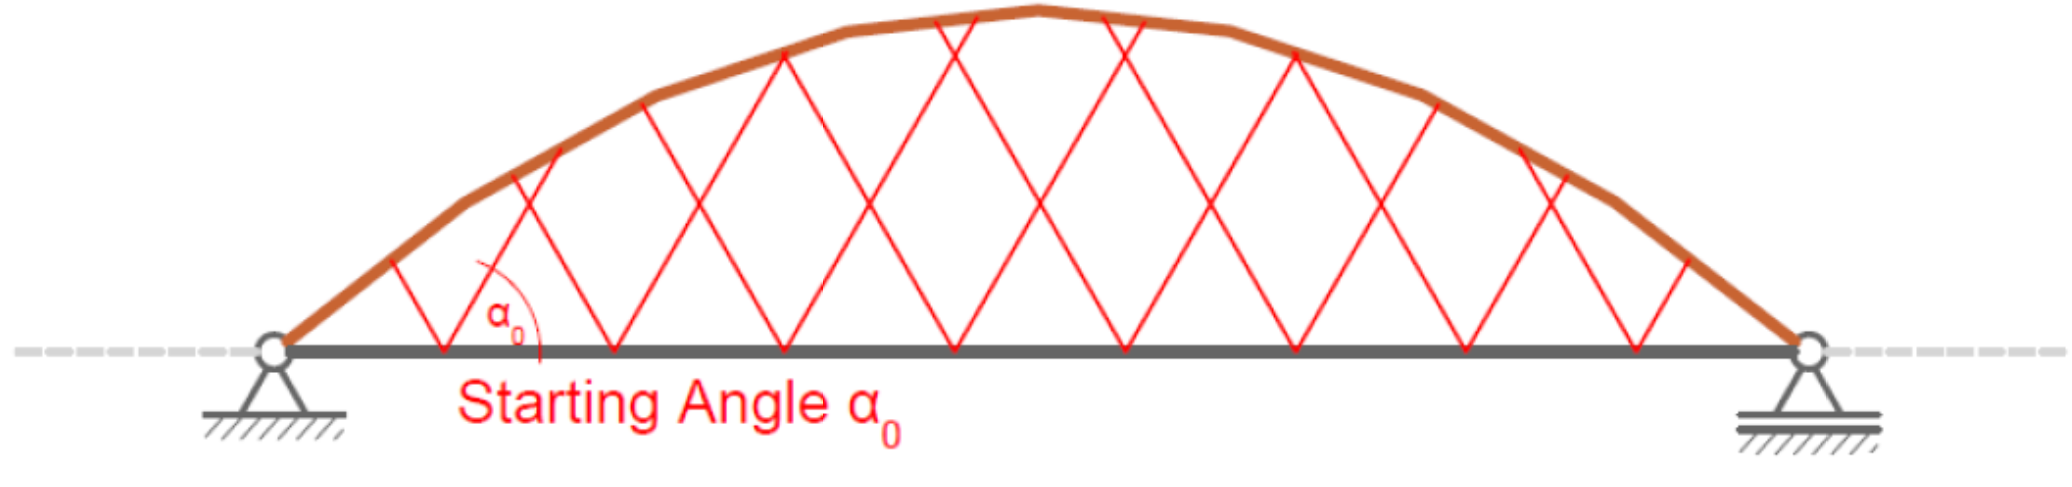
\includegraphics[width=0.9\textwidth]{Pictures/ParallelArrangementCavegn.PNG}
    \caption{Parallel arrangement}
    \label{fig:Cavegn2}
\end{subfigure}
\caption{Hanger arrangements and their parameters (adopted from \cite{Cavegn}).}
\label{fig:Cavegn}
\end{figure}

In the first step, the prestressing of the hangers was determined to minimize the bending moments under dead loads. To achieve this the hanger tuning matrix relating the individual unit strains of the hangers to their impacts was calculated using structural analysis software. This matrix was then used to calculate the prestrains giving minimal bending moments in the tie girder as shown in \autoref{fig:Cavegn3}. In a second step, the obtained normal forces were used to graphically construct the thrust line of the arch as illustrated in \autoref{fig:Cavegn4}. As the two steps influence each other, they are repeated until the obtained arch geometry does not change significantly. It was seen that the obtained arch geometries generally do not correspond to the circular or the parabolic shape. Sometimes they even lie outside of the two traditionally used shapes. By approximating the obtained shape with a quartic function an expression sufficiently close to the thrust line was found. Further, it was seen that flat angles of inclination lead to thrust lines that are more inclined near the bearing. Ultimately, the impacts under 3 live load combinations were used to estimate the costs of the generated structure which was taken as a further objective of the optimization. A flatter hanger inclination turned out to reduce the bending moment in the tie and the arch, whereas the opposite effect was observed in the maximum hanger forces. The estimated costs of the bridge were reduced the most by rapidly decreasing inclinations and high initial inclinations. The cost function was thereby minimized by up to 12\%. However also other patterns, e.g. with constant inclination, were shown to perform well if the arch geometry is adapted to the thrust line.
\begin{figure}[H]
\centering
\begin{subfigure}{0.5\textwidth}
    \centering
    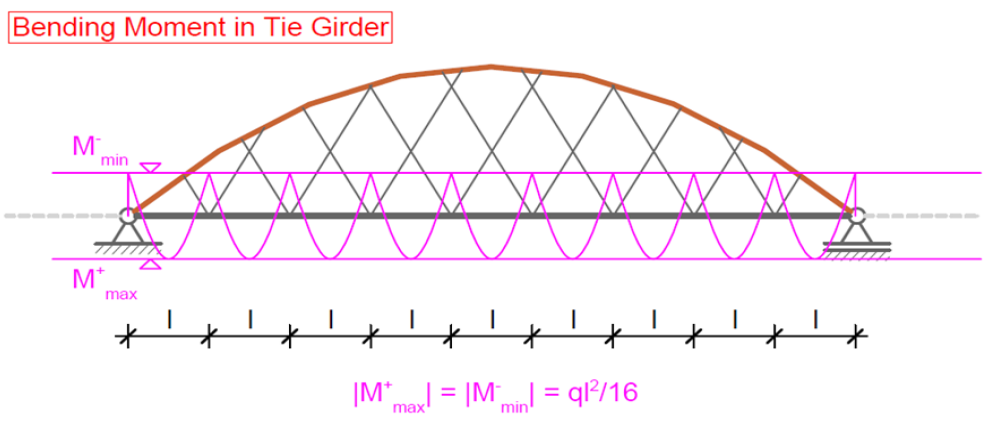
\includegraphics[width=0.73\textwidth]{Pictures/OptimizedBendingMoment.PNG}
    \caption{Determination of the self-equilibrium stress state}
    \label{fig:Cavegn3}
\end{subfigure}%
\begin{subfigure}{.5\textwidth}
    \centering
    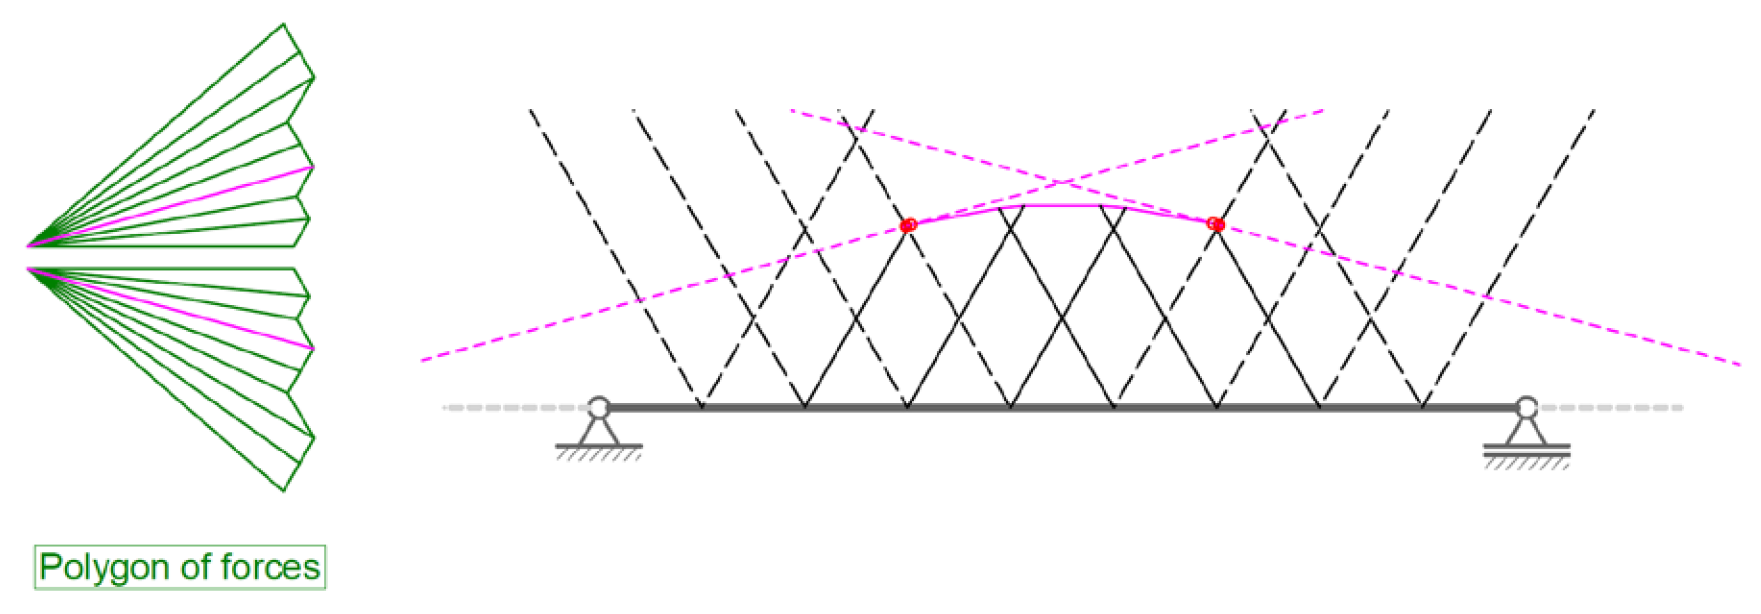
\includegraphics[width=0.9\textwidth]{Pictures/GraphicalThrustLineConstruction.PNG}
    \caption{Graphical construction of the arch shape}
    \label{fig:Cavegn4}
\end{subfigure}
\caption{Optimization steps (adopted from \cite{Cavegn}).}
\label{fig:Cavegn34}
\end{figure}

\newpage
\subsection{Summary} \label{sec:rev_sum}

Further it was pointed out early by \citep{Geissler} that only with a detailed structural model, including accurately modelled knuckles, reliable estimations of the hanger forces can be made.

In the last decade, many researchers have focused on the numerical optimization methods for given conditions. These methods produced efficient solutions for the structurally challenging problems. However, they do not provide practical help to the inexperienced engineer during the (preliminary) design. 
